\documentclass[journal=asbcd6,manuscript=article]{achemso}

\usepackage{natbib}
\usepackage{setspace}
\usepackage{xkeyval}
\usepackage{url}  % Formatting web addresses
\usepackage{ifthen}  % Conditional
\usepackage{multicol}   %Columns
\usepackage[utf8]{inputenc} %unicode support
\usepackage{amsmath}
\usepackage{amssymb}
\usepackage{mathtools}
\usepackage{epsfig}
\usepackage{epstopdf}
\usepackage{graphicx}
\usepackage{textcomp}
\usepackage{multirow}
\usepackage{booktabs}
\usepackage[margin=0.1pt,font=footnotesize,labelfont=bf]{caption}
\usepackage[version=3]{mhchem} % Formula subscripts using \ce{}
\usepackage[T1]{fontenc}       % Use modern font encodings
%\usepackage[square,sort,comma,numbers,sort&compress]{natbib}
%%%%%%%%%%%%%%%%%%%%%%%%%%%%%%%%%%%%%%%%%%%%%%%%%%%%%%%%%%%%%%%%%%%%%
%% If issues arise when submitting your manuscript, you may want to
%% un-comment the next line.  This provides information on the
%% version of every file you have used.
%%%%%%%%%%%%%%%%%%%%%%%%%%%%%%%%%%%%%%%%%%%%%%%%%%%%%%%%%%%%%%%%%%%%%
%%\listfiles

\bibliographystyle{achemso}
\newcommand*\mycommand[1]{\texttt{\emph{#1}}}

%%%%%%%%%%%%%%%%%%%%%%%%%%%%%%%%%%%%%%%%%%%%%%%%%%%%%%%%%%%%%%%%%%%%%
%% Meta-data block
%% ---------------
%% Each author should be given as a separate \author command.
%%
%% Corresponding authors should have an e-mail given after the author
%% name as an \email command. Phone and fax numbers can be given
%% using \phone and \fax, respectively; this information is optional.
%%
%% The affiliation of authors is given after the authors; each
%% \affiliation command applies to all preceding authors not already
%% assigned an affiliation.
%%
%% The affiliation takes an option argument for the short name.  This
%% will typically be something like "University of Somewhere".
%%
%% The \altaffiliation macro should be used for new address, etc.
%% On the other hand, \alsoaffiliation is used on a per author basis
%% when authors are associated with multiple institutions.
%%%%%%%%%%%%%%%%%%%%%%%%%%%%%%%%%%%%%%%%%%%%%%%%%%%%%%%%%%%%%%%%%%%%%
%%%%%%%%%%%%%%%%%%%%%%%%%%%%%%%%%%%%%%%%%%%%%%%%%%%%%%%%%%%%%%%%%%%%%
\author{Michael Vilkhovoy}
\author{Nicholas Horvath}
\author{Jeffrey D. Varner}
\email{jdv27@cornell.edu}
\phone{+1 607 2554258}
\fax{+1 607 2559166}
\affiliation[Cornell University]
{Robert Frederick Smith School of Chemical and Biomolecular Engineering, Cornell University, Ithaca, NY 14853}
%%%%%%%%%%%%%%%%%%%%%%%%%%%%%%%%%%%%%%%%%%%%%%%%%%%%%%%%%%%%%%%%%%%%%
\title{Analysis of Cell-Free Synthetic Circuits using Sequence Specific Constraints Based Modeling}
%\abbreviations{MV,NH,JDV}
\keywords{Synthetic biology, Constraints based modeling, Biochemical modeling}

%%%%%%%%%%%%%%%%%%%%%%%%%%%%%%%%%%%%%%%%%%%%%%%%%%%%%%%%%%%%%%%%%%%%%
%% The manuscript does not need to include \maketitle, which is
%% executed automatically.
%%%%%%%%%%%%%%%%%%%%%%%%%%%%%%%%%%%%%%%%%%%%%%%%%%%%%%%%%%%%%%%%%%%%%
\begin{document}

%%%%%%%%%%%%%%%%%%%%%%%%%%%%%%%%%%%%%%%%%%%%%%%%%%%%%%%%%%%%%%%%%%%%%
%% The "tocentry" environment can be used to create an entry for the
%% graphical table of contents. It is given here as some journals
%% require that it is printed as part of the abstract page. It will
%% be automatically moved as appropriate.
%%%%%%%%%%%%%%%%%%%%%%%%%%%%%%%%%%%%%%%%%%%%%%%%%%%%%%%%%%%%%%%%%%%%%
\begin{tocentry}

Some journals require a graphical entry for the Table of Contents.
This should be laid out ``print ready'' so that the sizing of the
text is correct.

Inside the \texttt{tocentry} environment, the font used is Helvetica
8\,pt, as required by \emph{Journal of the American Chemical
Society}.

The surrounding frame is 9\,cm by 3.5\,cm, which is the maximum
permitted for  \emph{Journal of the American Chemical Society}
graphical table of content entries. The box will not resize if the
content is too big: instead it will overflow the edge of the box.

This box and the associated title will always be printed on a
separate page at the end of the document.

\end{tocentry}

%%%%%%%%%%%%%%%%%%%%%%%%%%%%%%%%%%%%%%%%%%%%%%%%%%%%%%%%%%%%%%%%%%%%%
%% The abstract environment will automatically gobble the contents
%% if an abstract is not used by the target journal.
%%%%%%%%%%%%%%%%%%%%%%%%%%%%%%%%%%%%%%%%%%%%%%%%%%%%%%%%%%%%%%%%%%%%%
\begin{abstract}
In this study, we used sequence specific constraints based modeling to evaluate the performance of synthetic circuits in an \emph{E.~coli} TX-TL system.
A core \emph{E.~coli} metabolic model, consisting of XX metabolites and YY reactions, was developed from literature [REF].
This model, which described glycolysis, pentose phosphate pathway, amino acid biosynthesis and degradation and energy metabolism, was then augmented with
sequence specific descriptions of genetic circuits which included mechanistic models of promoter function, transcription and translation.
Thus, unlike other synthetic biology modeling efforts, sequence specific constraints based modeling explicitly couples
the transcription and translation of circuit components with the availability of metabolic resources.
Model parameters were largely taken from literature; our approach had very few adjustable parameters thereby allowing the a first principles prediction of circuit performance.
We tested this approach by first simulating $\sigma_{70}$-induced deGFP expression and then expanded these studies to more complex multicomponent circuits.
First principles predictions of circuit performance were consistent with measurements for a variety of cases.
Further, global sensitivity analysis identified the key metabolic processes that controlled circuit performance.
Taken together, sequence specific constraints based modeling offers a novel means to \emph{a~priori} estimate the performance of cell free synthetic circuits.
\end{abstract}

%%%%%%%%%%%%%%%%%%%%%%%%%%%%%%%%%%%%%%%%%%%%%%%%%%%%%%%%%%%%%%%%%%%%%
%% Start the main part of the manuscript here.
%%%%%%%%%%%%%%%%%%%%%%%%%%%%%%%%%%%%%%%%%%%%%%%%%%%%%%%%%%%%%%%%%%%%%
\section{Introduction}
Cell free systems offer many advantages for the study, manipulation and modeling of metabolism compared to \textit{in vivo} processes.
Central amongst these advantages is direct access to metabolites and the microbial biosynthetic machinery without the interference of a cell wall.
This allows us to control as well as interrogate the chemical environment while the biosynthetic machinery is operating, potentially at a fine time resolution.
Second, cell-free systems also allow us to study biological processes without the complications associated with cell growth.
Cell-free protein synthesis (CFPS) systems are arguably the most prominent examples of cell-free systems used today \cite{Jewett:2008aa}.
However, CFPS is not new; CFPS in crude \textit{E. coli} extracts has been used since the 1960s to explore fundamentally important biological mechanisms \cite{MATTHAEI:1961aa,NIRENBERG:1961aa}.
Today, cell-free systems are used in a variety of applications ranging from therapeutic protein production \cite{Lu:2014aa} to synthetic biology \cite{Hodgman:2012aa}.
Interestingly, many of the challenges confronting in-vivo genome-scale kinetic modeling can potentially be overcome in a cell-free system.
For example, there is no complex transcriptional regulation to consider, transient metabolic measurements are easier to obtain, and we no longer have to consider cell growth.
Thus, cell-free operation holds several significant advantages for model development, identification and validation.
Theoretically, genome-scale cell-free kinetic models may be possible for industrially important organisms, such as \textit{E. coli} or \textit{B. subtilis}, if a simple, tractable framework for integrating allosteric regulation with enzyme kinetics can be formulated.

Stoichiometric reconstructions of microbial metabolism popularized by constraint based modeling techniques such as flux balance analysis (FBA) have become standard tools to interrogate biological networks \cite{2012_lewis_palsson_NatRevMicrobio}.
Since the first genome-scale stoichiometric model of \textit{E. coli}, developed by Edwards and Palsson \cite{2000_edwards_palsson_PNAS}, stoichiometric reconstructions of hundreds of organisms, including industrially important prokaryotes such as \textit{E. coli} \cite{Feist:2007aa} or \textit{B. subtilis} \cite{Oh:2007aa}, are now available \cite{2009_feist_palsson_NatRevMicrobio}.
Stoichiometric models rely on a pseudo-steady-state assumption to reduce unidentifiable genome-scale kinetic models to an underdetermined linear algebraic system, which can be solved efficiently even for large systems using linear programming.
Traditionally, stoichiometric models have also neglected explicit descriptions of metabolic regulation and control mechanisms, instead opting to describe the choice of pathways by prescribing an objective function on metabolism.
Interestingly, similar to early cybernetic models, the most common metabolic objective function has been the optimization of biomass formation \cite{2002_ibarra_edwards_palsson_Nat}, although other metabolic objectives have also been estimated \cite{2007_schuetz_sauer_MolSysBio}.
Recent advances in constraint-based modeling have overcome the early shortcomings of the platform, including capturing metabolic regulation and control \cite{2013_hyduke_lewis_palsson_MolBioSys}. Thus, modern constraint-based approaches are extremely useful for the discovery of metabolic engineering strategies and represent the state of the art in metabolic modeling \cite{2013_mccloskey_palsson_feist_MolSysBio, 2012_zomorrodi_maranas_MetaEng}.

In this study, we used sequence specific constraints based modeling to evaluate the performance of synthetic circuits in an \emph{E.~coli} TX-TL system.
A core \emph{E.~coli} cell free metabolic model, consisting of XX metabolites and YY reactions, was developed from literature [REF].
This model, which described glycolysis, pentose phosphate pathway, amino acid biosynthesis and degradation and energy metabolism, was then augmented with
sequence specific descriptions of genetic circuits which included mechanistic models of promoter function, transcription and translation.
Thus, sequence specific constraints based modeling explicitly couples
the transcription and translation of circuit components with the availability of metabolic resources.
Model parameters were largely taken from literature; our approach had very few adjustable parameters thereby allowing the a first principles prediction of circuit performance.
We tested this approach by first simulating $\sigma_{70}$-induced deGFP expression and then expanded these studies to more complex multicomponent circuits.
First principles predictions of circuit performance were consistent with measurements for a variety of cases.
Further, global sensitivity analysis identified the key metabolic processes that controlled circuit performance.
Taken together, sequence specific constraints based modeling offers a novel means to \emph{a~priori} estimate the performance of cell free synthetic circuits.

\section{Results and discussion}


\section*{Results}
\subsection{Model Derivation}
The goal of this work was first to construct a modeling framework to describe cell-free protein synthesis systems and to examine its performance in productivity and yield for a protein of interest.
One mathematical framework that has found wide use in modeling metabolism are constraint based models such as flux balance analysis (FBA).
FBA can predict how cells utilize nutrients to produce products by using the biochemical stoichiometry and thermodynamical feasibility under pseudo steady-state conditions.
Traditionally, FBA is used to model \textit{in vivo} processes, however cell-free systems do not have growth associated reactions or transport through the cell membrane.
Thus, to model cell-free metabolism we constructed a cell-free stoichiometric network by removing growth associated reactions from the MG1655 reconstruction \cite{Feist:2007aa}, and incorporating amino acid synthesis and transcription/translation associated reactions \cite{Allen:2003aa} for a protein of interest to be expressed. 
The network consisted of 281 reactions and 132 species. 
We developed a cell-free sequence specific flux balance analysis (ssFBA) with a detailed promoter model \cite{Moon:2012aa} to examine the performance of CFPS. 
We first validated the ssFBA approach by comparing simulated and measured concentrations of two proteins from two different cell-free \textit{E. coli} extract systems.
The first protein, chloramphenicol acetyltransferase (CAT), was produced under a T7 promoter in a glucose/NMP cell-free system \cite{2005_calhoun_BiotechnologyProgress} for a duration of 1 hour under glucose consumption (Fig \ref{fig:CAT_GFP_prod}A).
The second protein, dual emission green fluorescent protein (deGFP), was produced under a P70 promoter in TXTL 2.0 \textit{E. coli} extract for a duration of 8 hours under maltose consumption(Fig \ref{fig:CAT_GFP_prod}B).
The ssFBA simulations predicted the production of both proteins for the duration of both CFPS batch reactions.
Uncertainty in experimental factors such as RNA polymerase, ribosome concentrations, elongation rates or the upper bounds for oxygen and glucose consumption rates did not alter the qualitative performance of the model. 
Thus, the metabolic network and molecular description of trancription and translation were consistent with experimental measurements.
\begin{figure}[t!]
\centering
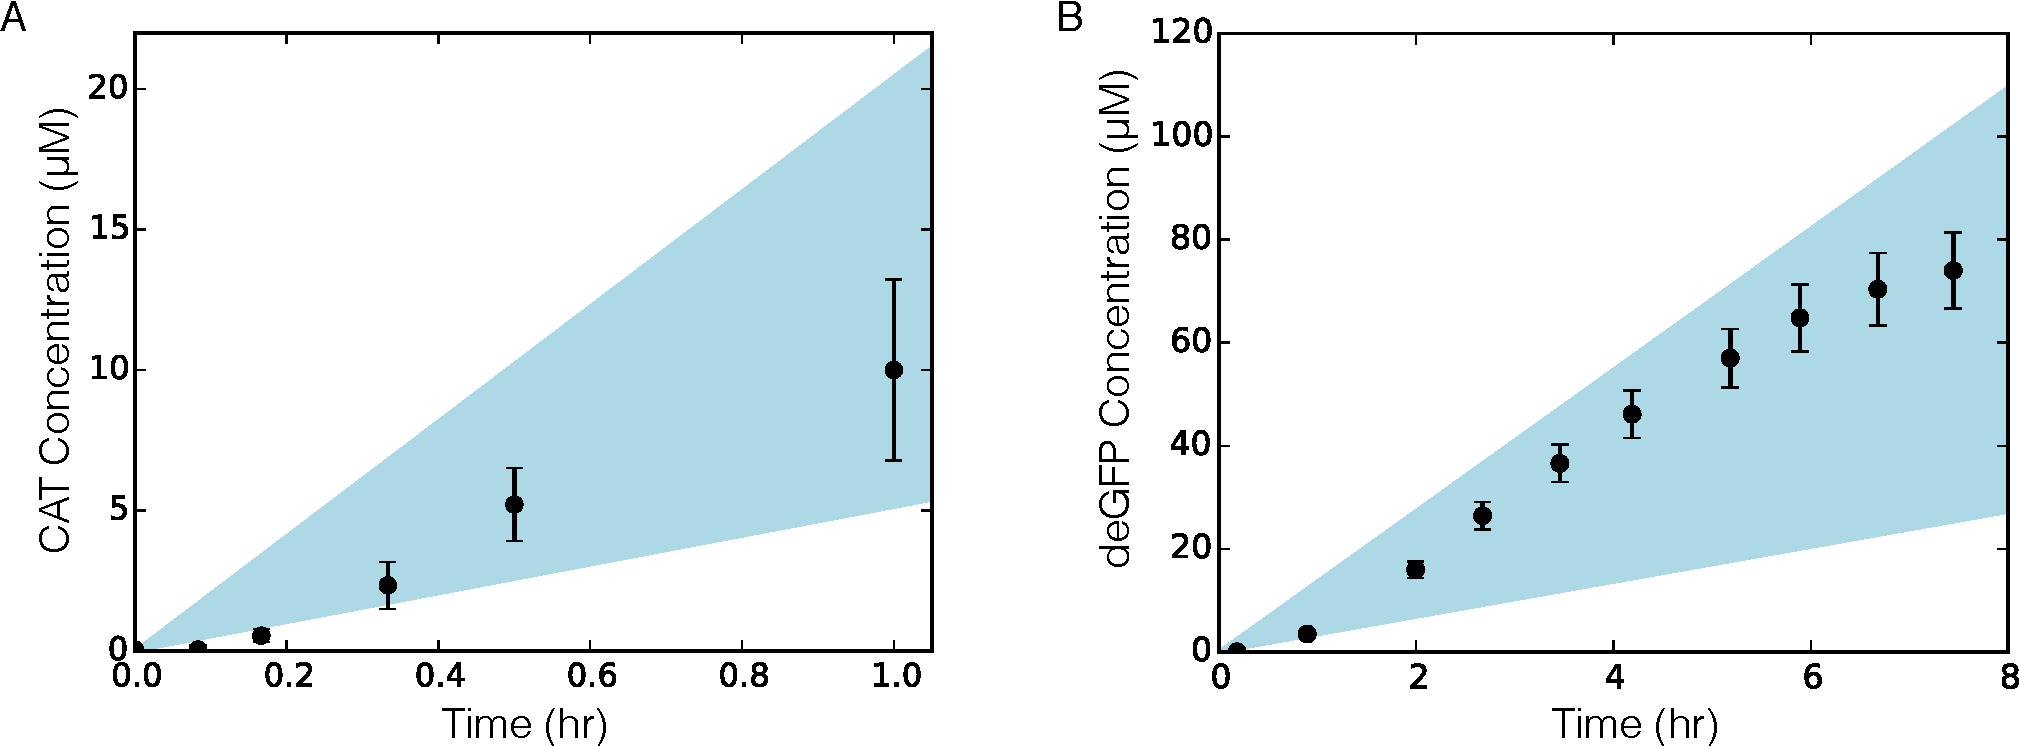
\includegraphics[width=1.00\textwidth]{./Figures/CAT_GFP_prod.pdf}
\caption{Sequence specific flux balance analysis of protein production vesus time. A. CAT production under a T7 promoter in CFPS \textit{E. coli} extract for 1 hr under glucose consumption. B. deGFP production under a P70 promoter in TXTL 2.0 \textit{E. coli} extract for 8 hr under glucose consumption. 95\% CI (blue region) over the ensemble of 100 sets.}
\label{fig:CAT_GFP_prod}
\end{figure}

Next, ssFBA predicted deGFP production as a function of plasmid concentration (Fig \ref{fig:GFP_plasmid}).
Concentration of deGFP at each plasmid concentration was calculated by multiplying the flux of deGFP synthesis by the active time of production, approximately 8 hours in TXTL 2.0 \cite{2016_Garamella_etal_TXTL}. 
The mean of the ensemble shows a good prediction against the measured deGFP levels, even though it under predicted deGFP concentration at the saturating point of 5 nM of plasmid concentration.  
However, the ensemble and the mean of the ensemble captured the overall saturating dynamics of deGFP production as a function of plasmid concentration.
\begin{figure}[t!]
\centering
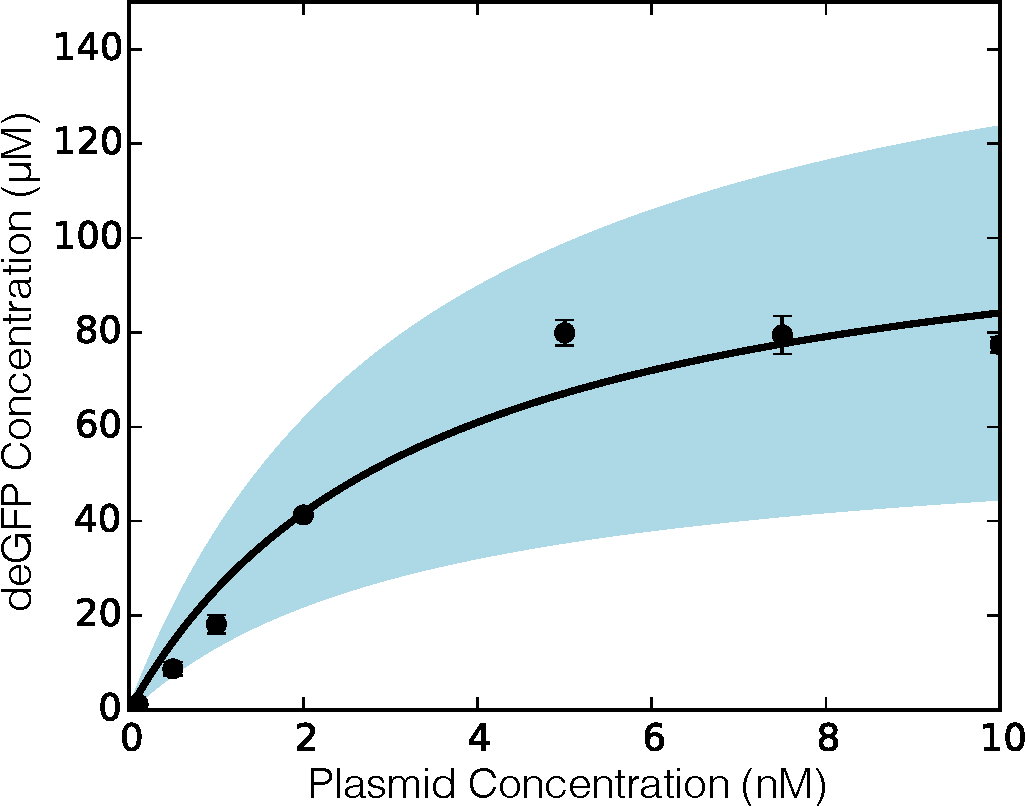
\includegraphics[width=0.6\textwidth]{./Figures/GFP_plasmid.pdf}
\caption{Predicted deGFP concentration (black line) at different plasmid concentrations versus measurements of deGFP (dots) synthesized in TXTL 2.0. 95\% CI (blue region) over the ensemble of 100 sets.}
\label{fig:GFP_plasmid}
\end{figure}

These results validated our mathematical framework to model CFPS systems and predict the production of two proteins with no adjustable parameters. 
It also showed that the sequence specific reactions were sufficient to predict the production of two different proteins under different promoters and cell-free systems. 
Since the model accurately predicted the behavior of protein production, we wanted to use our mathematical framework to help us understand the performance limits of CFPS and how these shortcomings could be addressed. 

\subsection{Examining CFPS Performance: Productivity}
Our next goal was to examine the performance of CFPS productivity for eight different proteins under three different cases. Each of the proteins were produced under a P70 promoter, except for CAT which was produced under a T7 promoter. In all our cases, CFPS is supplied with glucose. The first case, CFPS is supplied with amino acids and the system can synthesis amino acids (control). In the second case, CFPS is supplied with amino acids, however the system cannot synthesis amino acids (AA uptake w/o synthesis). We turned off these synthesis reactions because during the cell-free extract preparation the cells are often supplied with amino acids, thus the enzymes responsible for amino acid synthesis would not be present. In the third case, CFPS is not supplied with amino acids, but the system can synthesis them (AA synthesis w/o uptakte).    
We used ssFBA to estimate the productivity of eight proteins for each case (Fig \ref{fig:Prod_POI}A).
The second case (without amino acid synthesis) showed the highest productivity for each of the proteins, however the control case had very similar performance.
This shows the system has sufficient substrates to power the system and synthesis each protein. 
The third case had the lowest productivity for each protein, thus the addition of amino acids to CFPS extract is important for maintaining a relatively high productivity.
The qualitative trend of productivity for the three different cases was the same, however some proteins had higher productivity than others. 
For instance, in the second case FGF21 had a productivity of 17 ($\mu$M/h) whereas FII had a productivity of 3 ($\mu$M/h).
To examine this further, the mean productivity was plotted against the carbon number of each protein (Fig \ref{fig:Prod_POI}B).
The proteins with the highest productivity had the lowest carbon number whereas proteins with low productivity had higher carbon numbers.     
This inverse qualitative trend was due to the fact that larger proteins require more amino acids and substrates to assemble them resulting in lower productivity. 
\begin{figure}[t!]
\centering
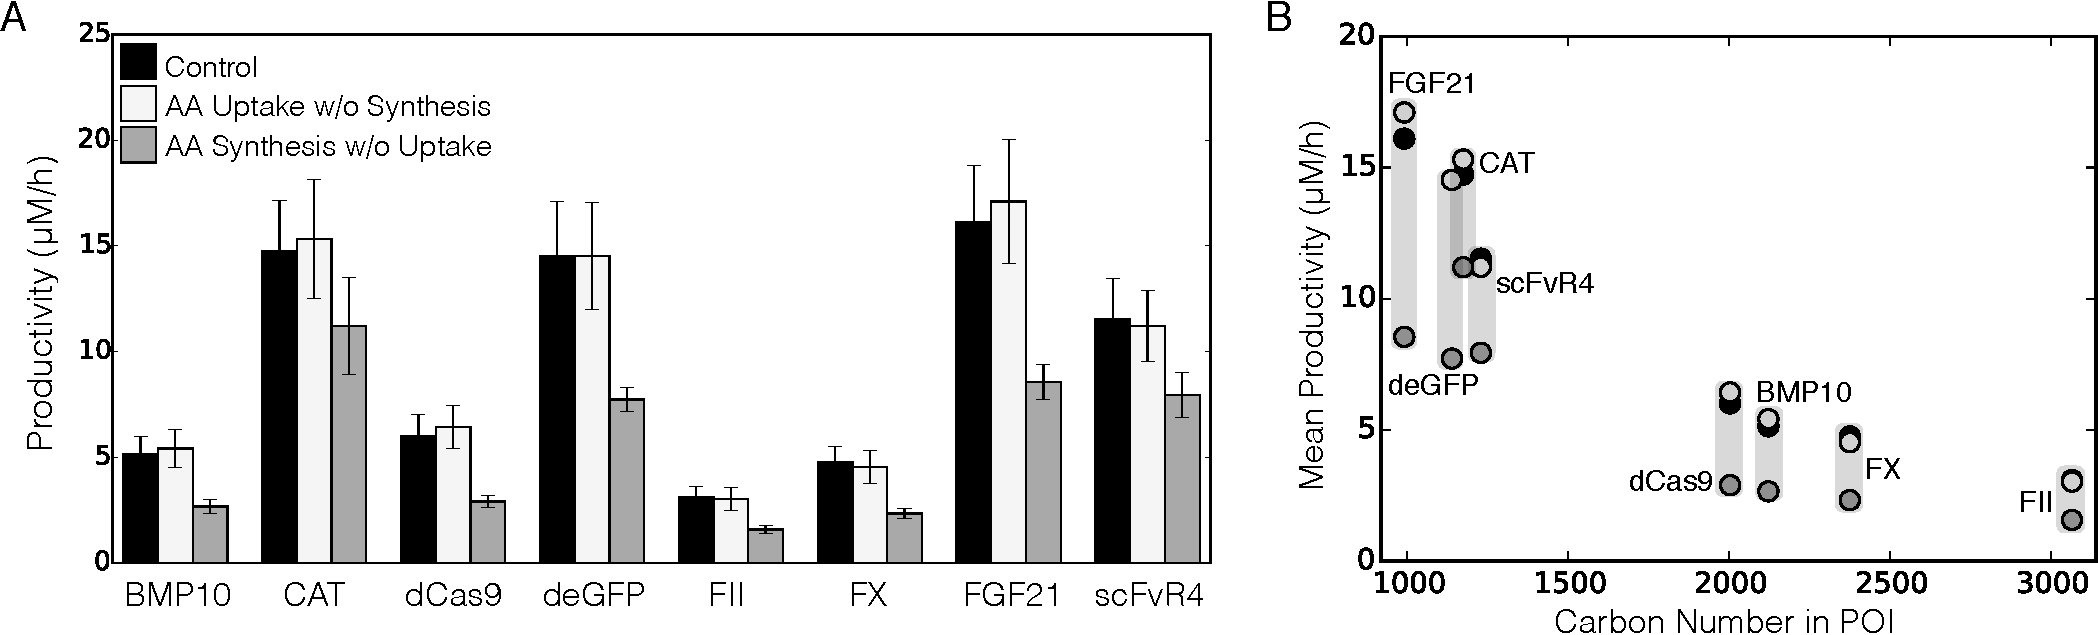
\includegraphics[width=1.00\textwidth]{./Figures/Prod_POI.pdf}
\caption{CFPS productivity performace for eight proteins for the control (black), AA uptake w/o synthesis (off white), and AA synthesis w/o uptake (grey). A. Productivity normalized to the specific glucose uptake rate (Error bars represent the 95\% CI of the ensemble). B. Mean productivity versus the carbon number for each corresponding protein.}
\label{fig:Prod_POI}
\end{figure}

\subsection{Examining CFPS Performance: Carbon Yield}
Following the same outline as in examining the productivity, we calculated the carbon yield for each protein (Fig \ref{fig:Yield_POI}A). 
The same trends followed, where the case without amino acid synthesis showed the highest carbon yield and the control case had comparable performance. 
The third case (with no amino acid uptake) had the lowest yields; this is most likely because glucose is now utilized to synthesize the necessary amino acids for each protein as well as power the system. 
Interestingly, CAT carbon yield showed similar performance for all three cases. 
Each protein has different energy requirements for transcription and translation depending on its sequence.
Thus, for the case of CAT, energy requirements for transcription or translation are low enough that it's carbon yield is not hindered in the third case.
We next investigated the effect of the carbon number of each protein to the carbon yield (Fig \ref{fig:Yield_POI}B). 
The same inverse qualitative trend is observed, however it is less significant. 
Sequence specific flux balance analysis assumes a psuedo steady state, thus intermediate metabolites cannot be accumulated within the cell-free extract.
In addition, ssFBA is solved by setting the production of the protein as the objective function.
Therefore, carbon flux will travel throughout the network to optimize the flux through the protein synthesis reaction. 
This leads to slightly similar carbon yields for all the proteins, however, the lower carbon number protein still observe a higher carbon yield.  
\begin{figure}[t!]
\centering
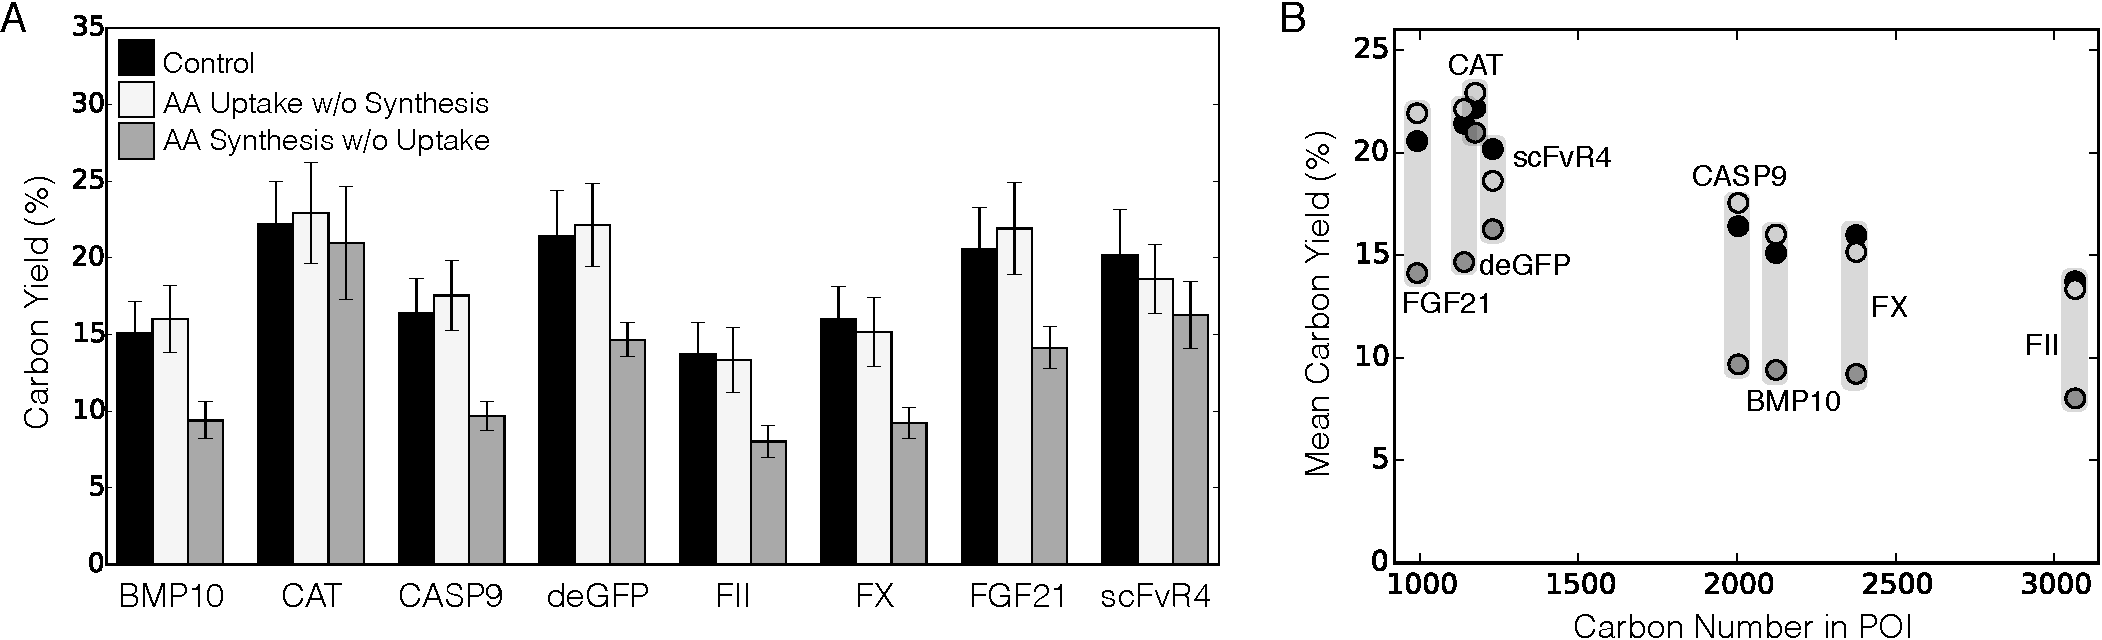
\includegraphics[width=1.00\textwidth]{./Figures/Yield_POI.pdf}
\caption{CFPS carbon yield performace for eight proteins for the control (black), AA uptake w/o synthesis (off white), and AA synthesis w/o uptake (grey). A. Carbon yield (Error bars represent the 95\% CI of the ensemble). B. Mean carbon yield versus the carbon number for each corresponding protein.}
\label{fig:Yield_POI}
\end{figure}


\subsection{Sensitivity analysis on CFPS Performance}
To better understand the effect of substrate utilization and transcription/translation parameters on CFPS performance we performed global sensitivity analysis on productivity and carbon yield for deGFP, a representative protein (Fig \ref{fig:SI_GFP}).
In examining productivity performance (Fig \ref{fig:SI_GFP}A), the significance of transcription/translation parameters were fairly constant across all three cases, with the elongation rate by ribosomes being the most sensitive.
This shows the rate of translation is instrumental in achieving high productivity, and should be the first step to investigate in order to optimize productivity, prior to examining transcription rates, this is consistent with literature findings.
Underwood and coworkers have also shown that an increase in ribosome levels does not significantly increase protein yields or rates; however, adding elongation factors increased yields by 23\% at 30 minutes \cite{2005_underwood_biotech}.
In addition, Li et al. have increased productivity of firefly lucifease by 5-fold in CFPS systems by adding and adjusting factors that affect transcription and translation such as elongation factors, ribosome recyclcing factor, release factors, chaperones, BSA, and tRNAs \cite{2014_li_PlosOne}.
In examining the substrate utilization, glucose uptake was not very important for productivity in the first two cases, but its significance increased when amino acids was removed from CFPS.
This makes sense, as amino acid synthesis can only come from glucose and becomes the only way to power protein synthesis.
On the other hand, when amino acid synthesis is removed, amino acid uptake becomes more important, as it becomes the only source of amino acids.
\begin{figure}[t!]
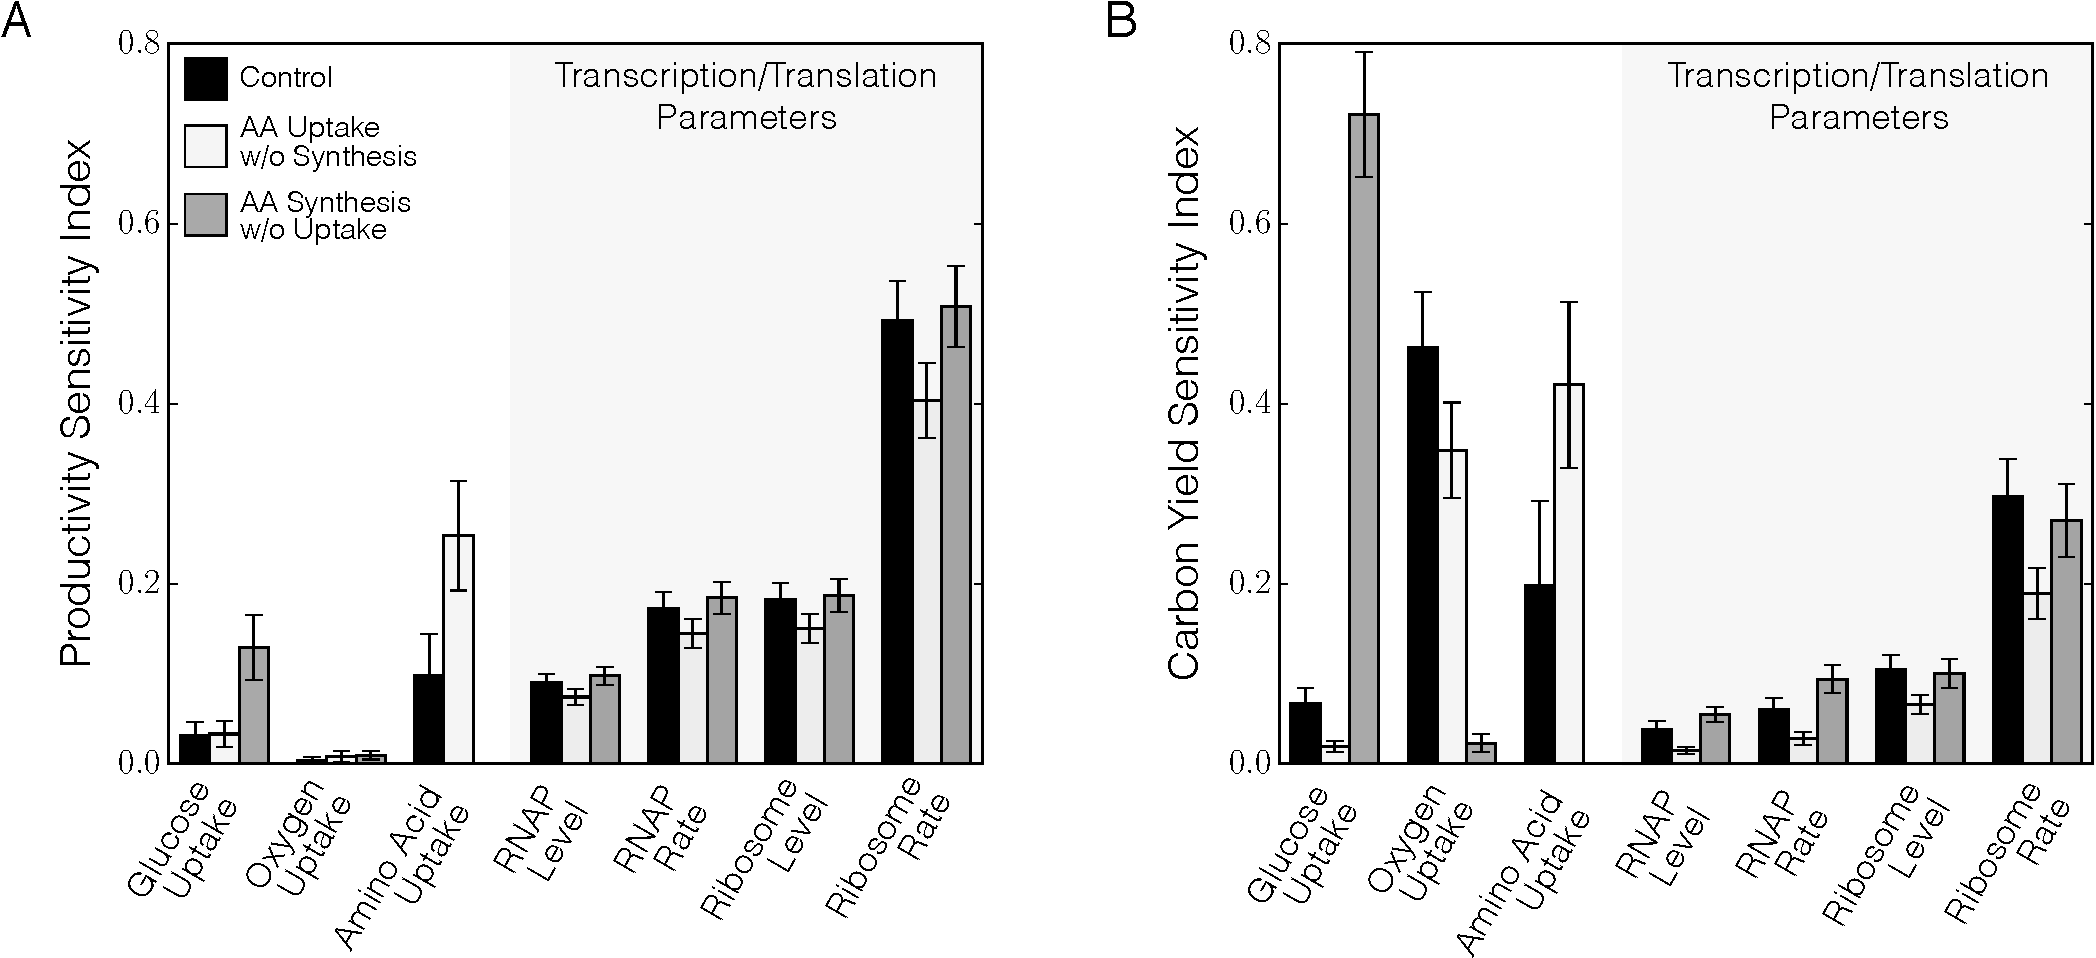
\includegraphics[width=1.00\textwidth]{./Figures/SI_GFP.pdf}
\caption{Total order sensitivity of deGFP productivity (A) and carbon yield (B) to specific uptake rates and transcription/translation parameters for three cases: control (black), amino acid uptake without synthesis (off white), and amino acid synthesis without uptake (gray). (Error bars represent 95\% CI of the ensemble).}
\label{fig:SI_GFP}
\end{figure}

When considering carbon yield performance (Fig \ref{fig:SI_GFP}B), the substrate and oxygen uptake fluxes become much more important while the sensitivity to kinetic parameters decreases slightly.
This is likely because glucose and oxygen uptake determine the mechanism of energy generation, which is critical to efficient protein production.
Meanwhile, productivity is determined primarily by the rate of the most downstream steps, transcription and translation.
Interestingly, in the first two cases, oxygen uptake has a significant effect on carbon yield.
This is most likely due to the importance of oxidative phosphorylation for efficient energy generation.
However, in the third case (with no amino acid uptake), oxygen uptake becomes insignificant compared to the other parameters, while glucose uptake becomes the most siginificant.  
This may be because glucose is required for both amino acid synthesis and efficient energy generation, both of which are important for a high yield.
Thus, there is a tradeoff between energy generation to power transcription/translation as well as synthesize amino acids which are required to assemble the protein of interest. 
Across all three cases, substrate utilization (amino acid uptake and glucose) showed to be the next important as these substrates are contributing to the carbon yield of deGFP.
The transcription/translation parameters had the same trend as in the productivity trend, where the ribosome elongation rate was the most sensitive compared to the transcription/translation parameters and showed significant importance across all parameters. 
Thus, in investigating CFPS performance of productivity and yield, the ribosome elongation rate seems to be an important parameter to optimize, as been already shown in literature \cite{2005_underwood_biotech, 2014_li_PlosOne}. 

We also performed this sensitivity analysis on CAT production, which did not show the same trend in yield across the three cases as the other proteins.
For CAT, glucose uptake was as important to productivity as the kinetic parameters.
Also, the increase in amino acid uptake importance to both productivity and yield was much greater.
Finally, oxygen uptake became the most important factor in yield and maintained this across all three cases.
Apart from these differences, the general trend of transcription and translation mattering more for productivity and uptake mattering more for yield was still true.




\begin{figure}[t!]
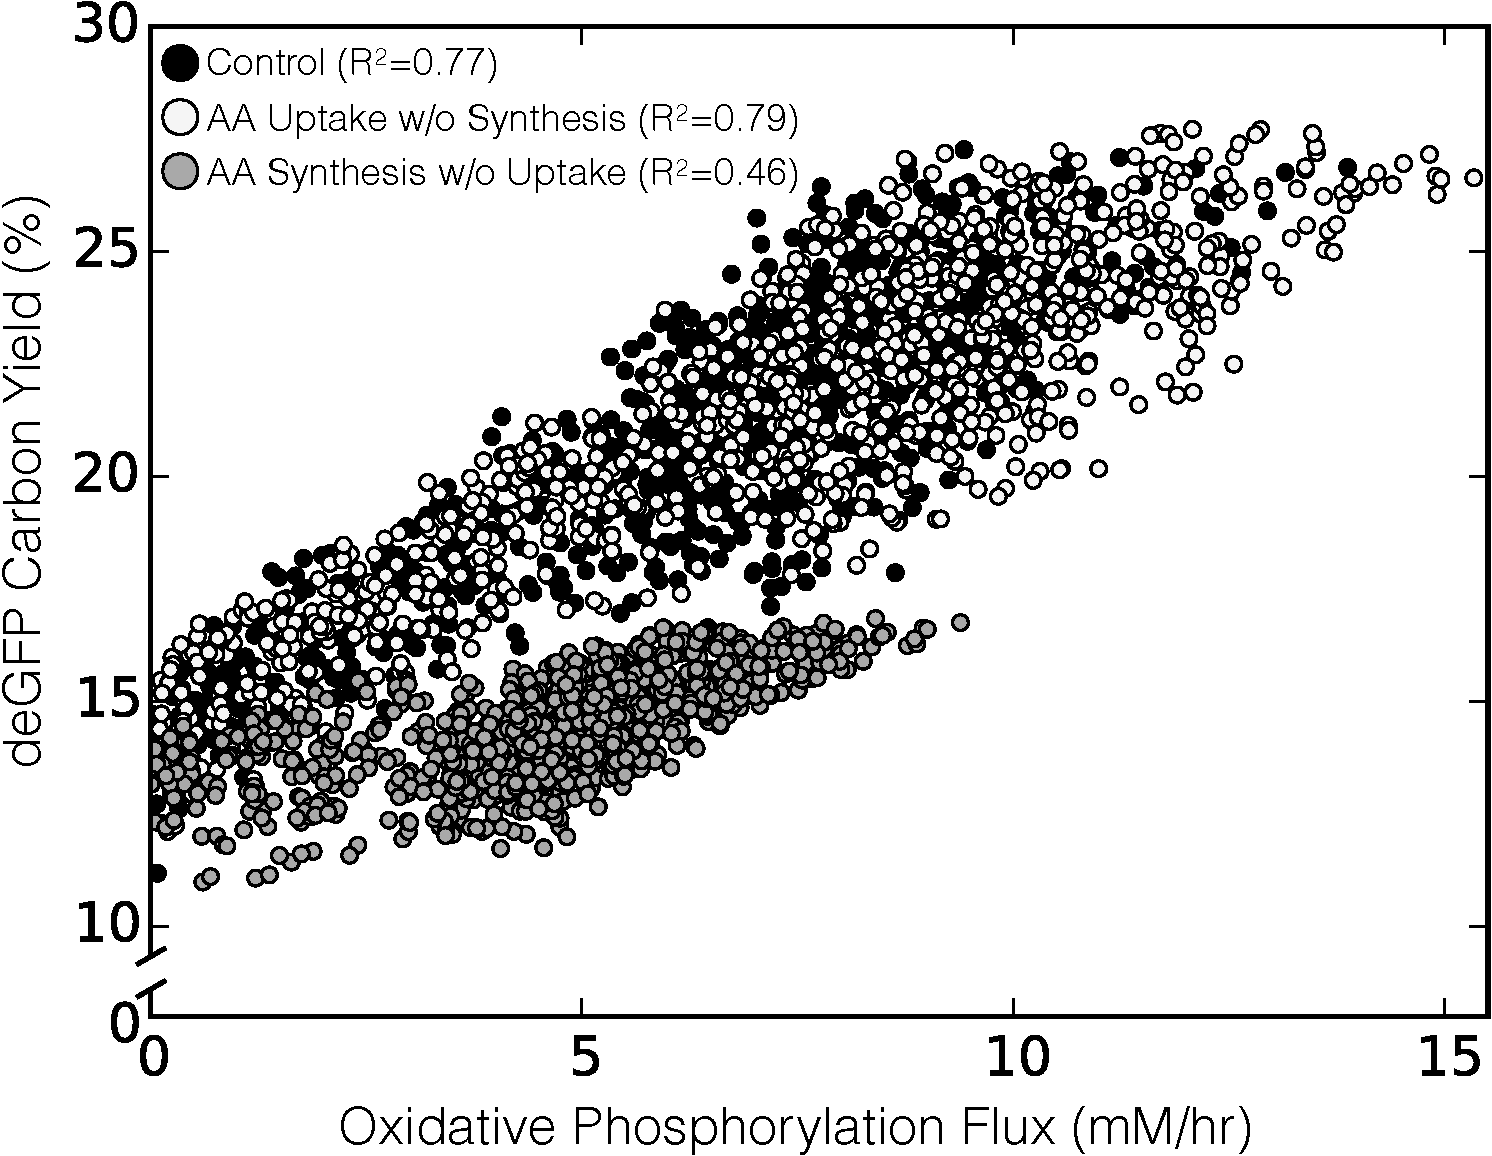
\includegraphics[width=0.7\textwidth]{./Figures/OxPhos_yield.pdf}
\caption{An ensemble of 1000 ssFBA solutions for deGFP carbon yield versus oxidative phosphorylation flux for three cases: control (black), amino acid uptake without synthesis (off white), and amino acid synthesis without uptake (gray). }
\label{fig:oxphos}
\end{figure}

\begin{figure}[t!]
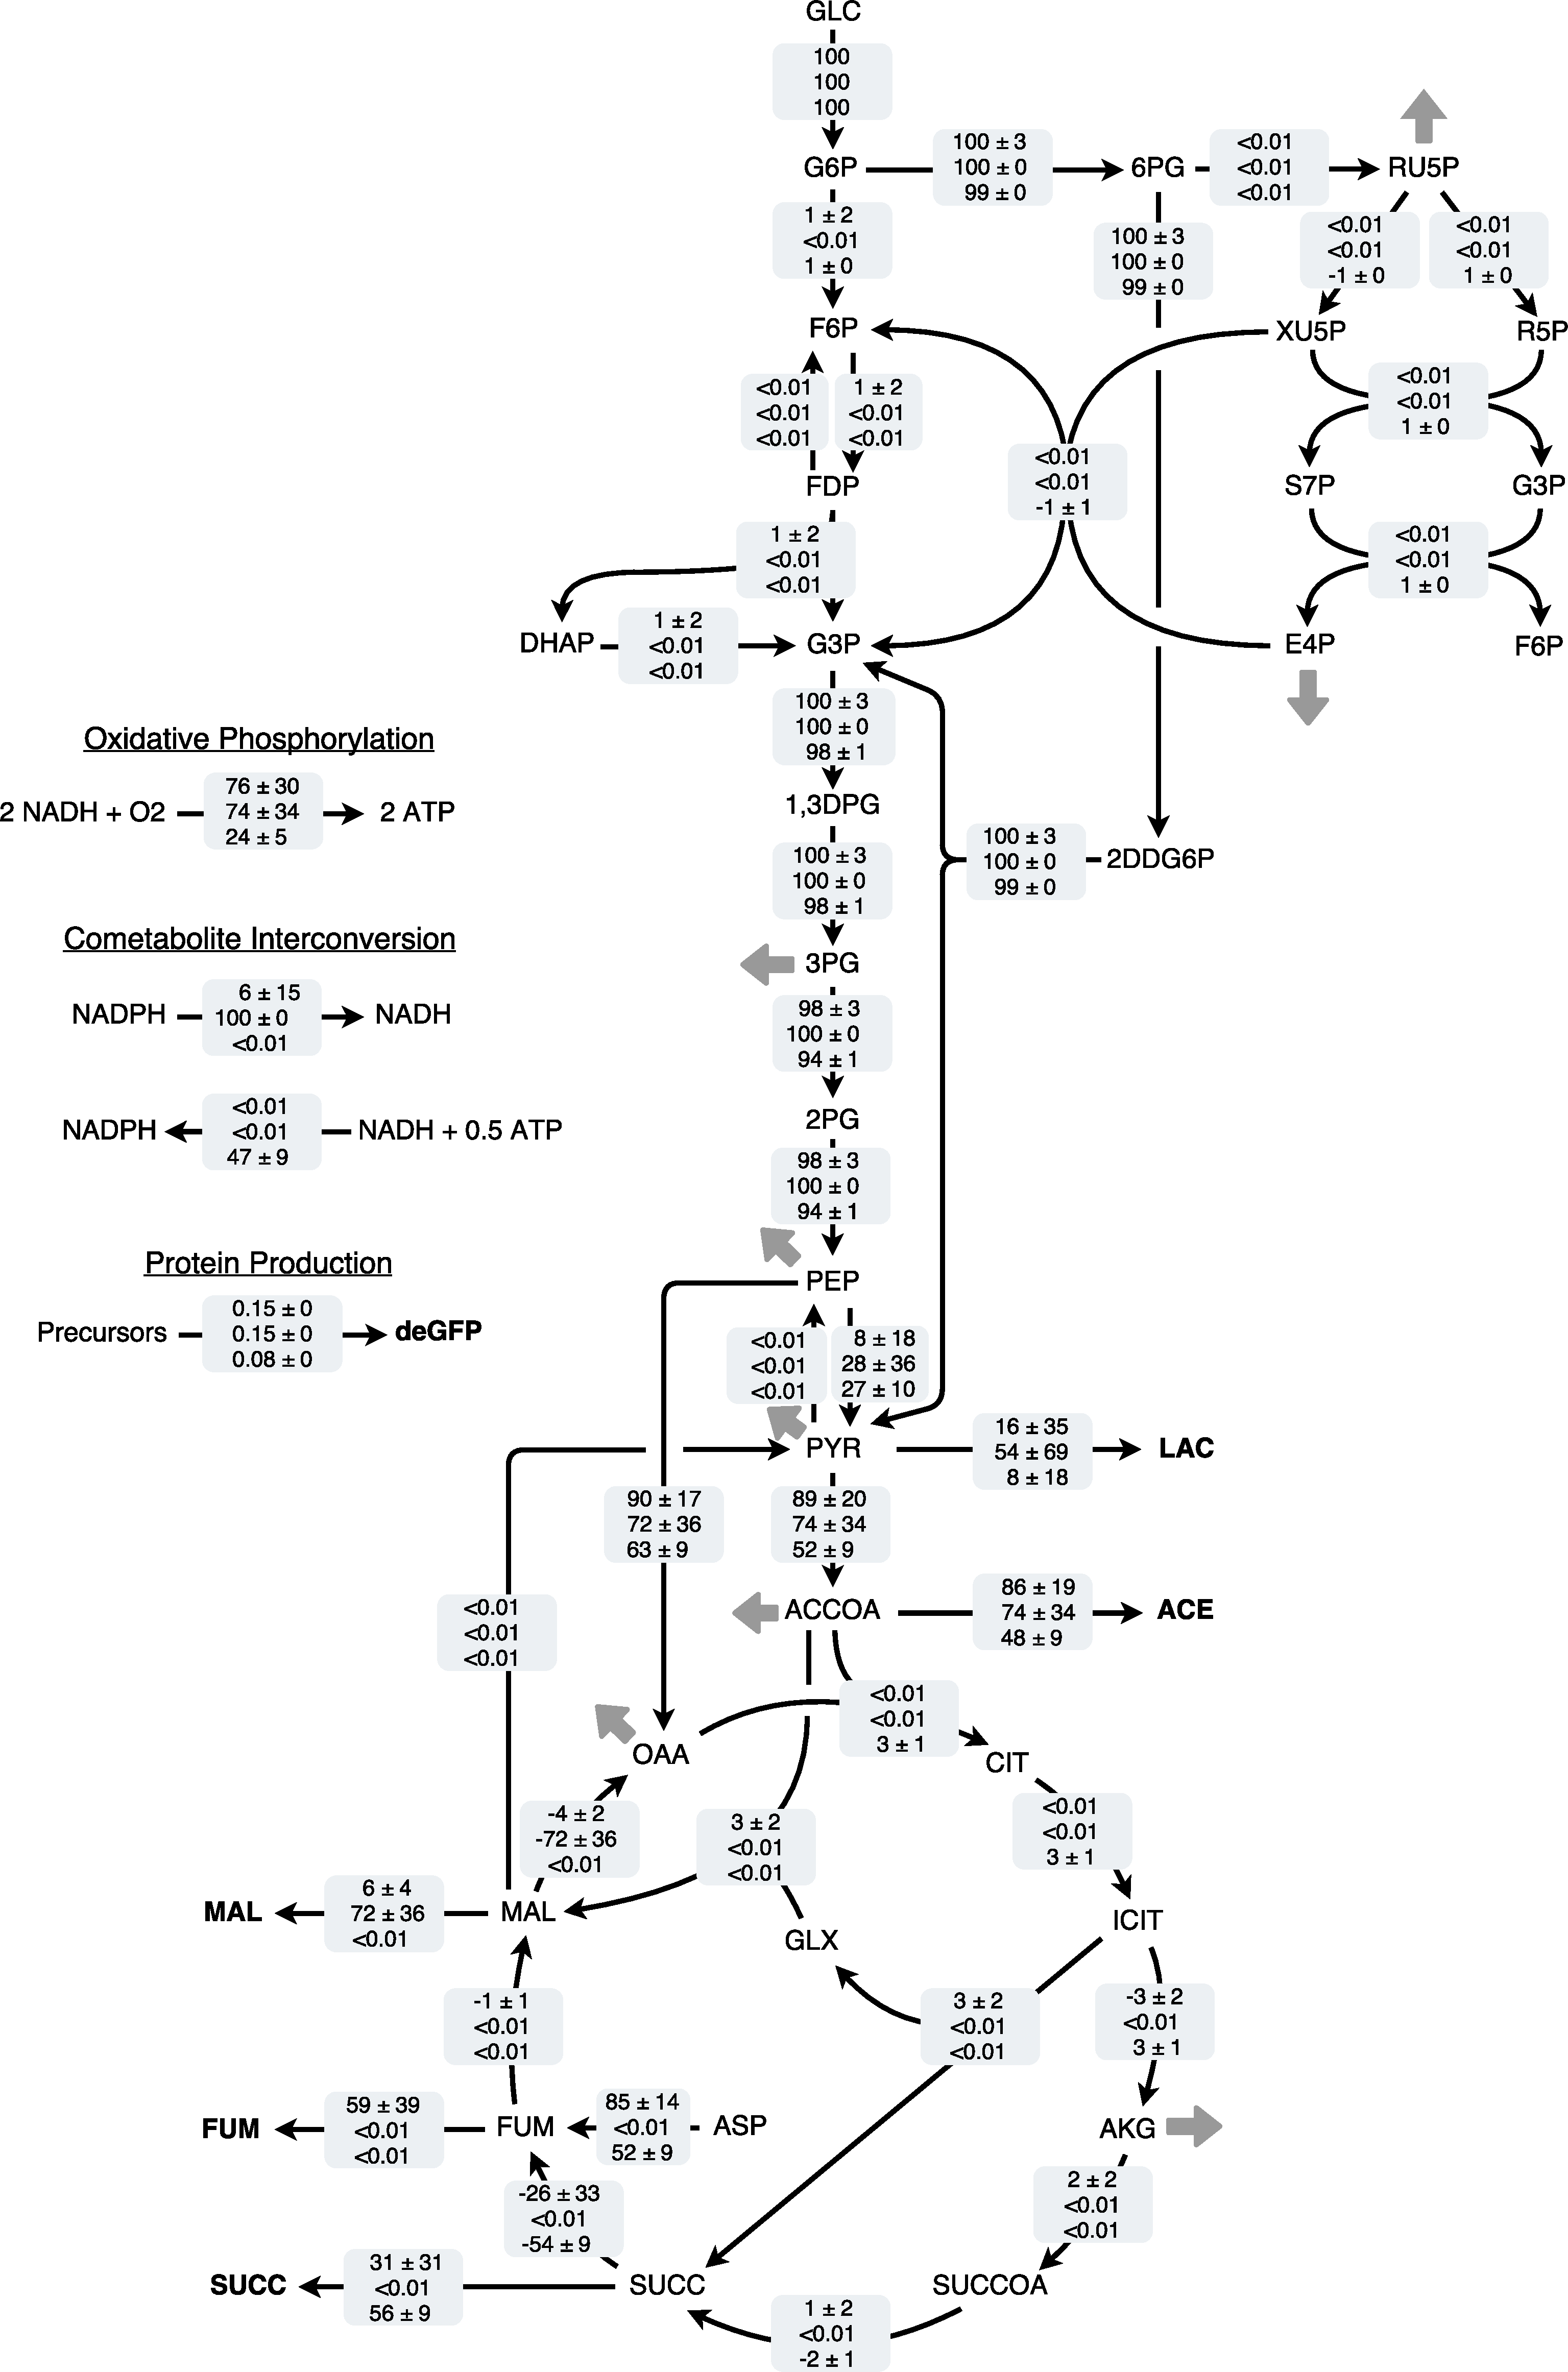
\includegraphics[width=0.8\textwidth]{./Figures/flux.pdf}
\caption{deGFP production flux profile for glycolysis, pentose phosphate pathway, Entner-Doudoroff pathway, TCA cycle, NADPH/NADH transfer, and oxidative phosphorylation. Flux (mean $\pm$ standard deviation) across ensemble normalized to glucose uptake flux. Flux distribution for three different cases: control (top row), amino acid uptake without synthesis (second row), and amino acid synthesis without uptake (third row). Bold metabolites are allowed to accumulate; grey arrows lead to amino acid synthesis.}
\label{fig:flux}
\end{figure}


\begin{figure}[t!]
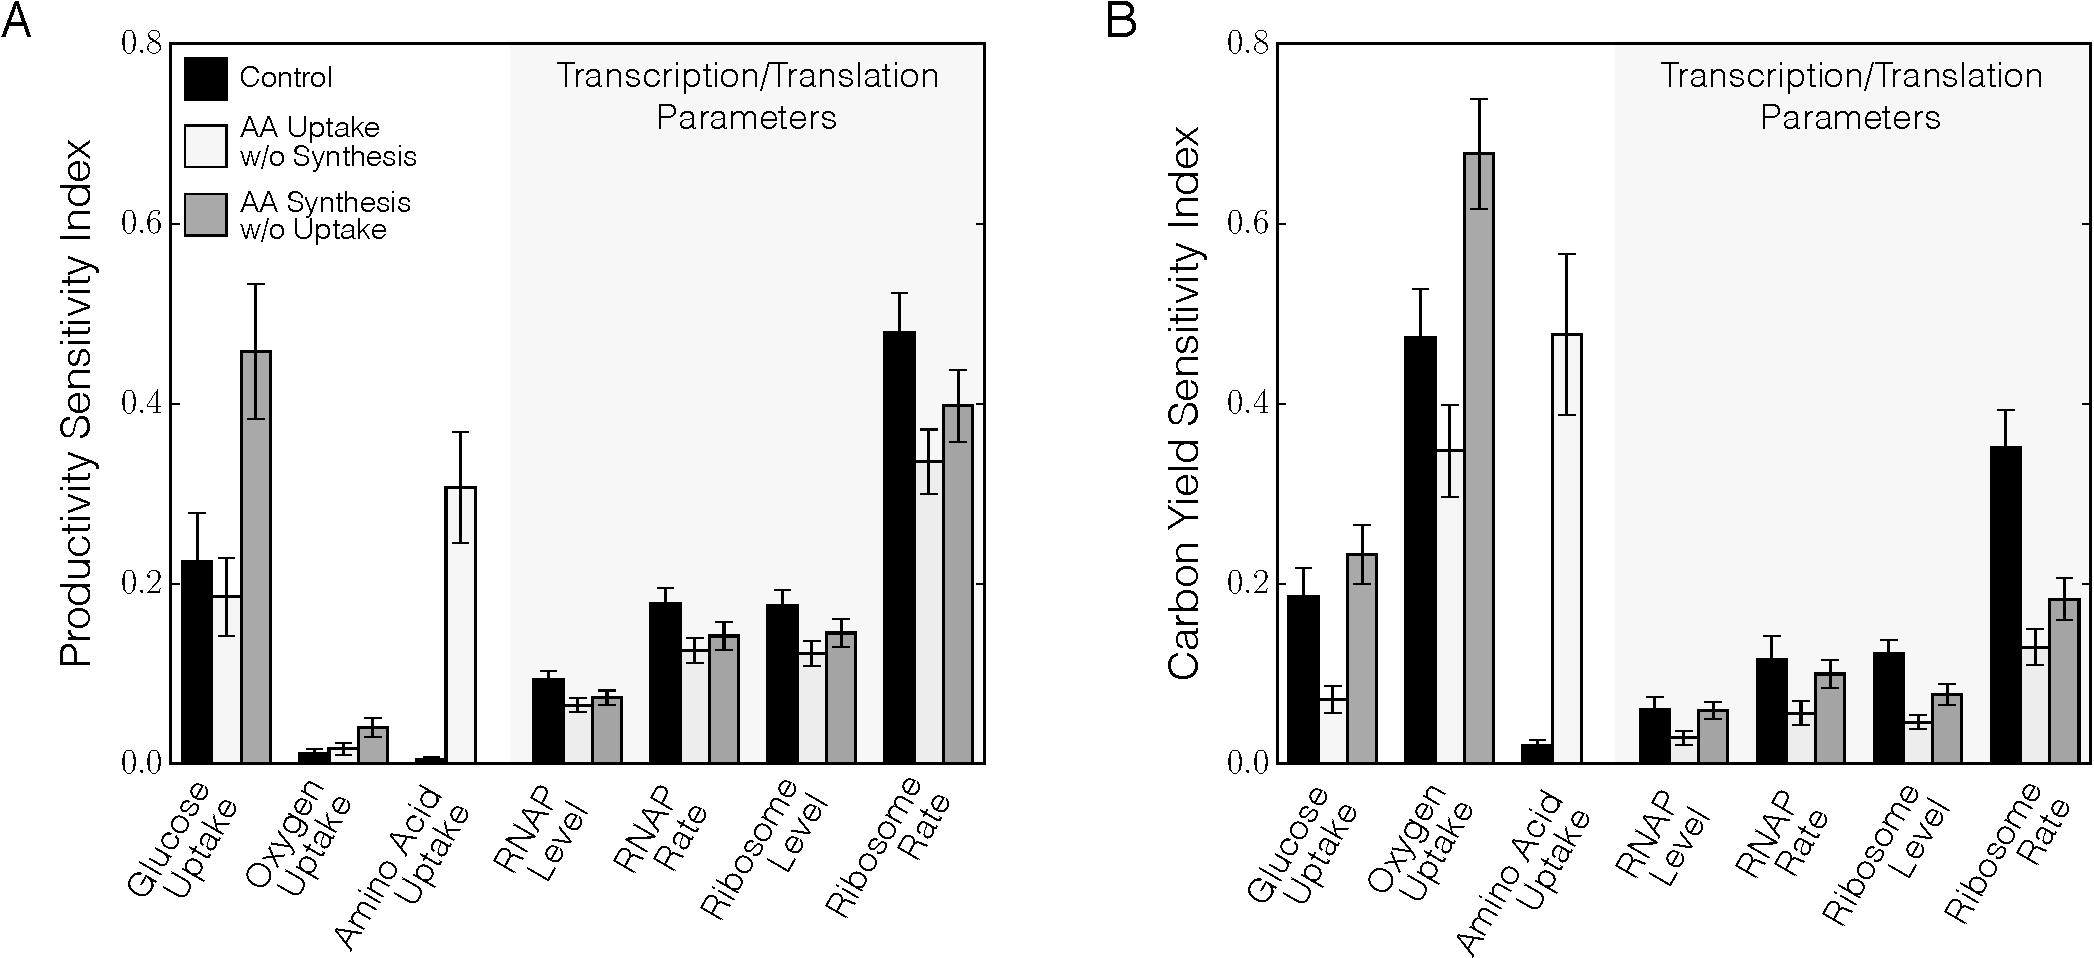
\includegraphics[width=1.00\textwidth]{./Figures/SI_CAT.pdf}
\caption{Total order sensitivity of CAT productivity (A) and carbon yield (B) to specific uptake rates and transcription/translation parameters for three cases: control (black), amino acid uptake without synthesis (off white), and amino acid synthesis without uptake (gray). (Error bars represent 95\% CI of the ensemble).}
\label{fig:SI_CAT}
\end{figure}



\begin{table}%[h]
\centering
    \caption{Carbon contribution from glucose and each amino acid toward deGFP production for three cases: control, amino acid uptake without synthesis, and amino acid synthesis without uptake.}
    \renewcommand{\arraystretch}{0.95}
    \begin{tabular}{lccc} \toprule
        \parbox{3.2 cm}{Carbon \phantom{abcdefghi} Produced (mM)} & Control & \parbox{2.5 cm}{AA uptake \phantom{ai} w/o synthesis} & \parbox{2.5 cm}{AA synthesis w/o uptake} \\ \midrule
        deGFP & 9.8 & 9.6 & 9.9  \\ \toprule
        \parbox{3.2 cm}{Carbon \phantom{abcdefghi} Consumed (mM)} & \\ \midrule
        GLC & 37.3 & 33.7 & 66.9 \\ 
        ALA & 0.0 & 0.2 & -  \\ 
        ARG & 0.3 & 0.3 & - \\ 
        ASN & 0.5 & 0.4 & -  \\ 
        ASP & 0.4 & 0.6 & -  \\ 
        CYS & 0.2 & 0.1 & -  \\ 
        GLU & 2.1 & 0.6 & -  \\ 
        GLN & 0.4 & 0.3 & - \\ 
        GLY & 0.3 & 0.3 & -  \\
        HIS & 0.5 & 0.5 & - \\
        ILE & 0.0 & 0.6 & -  \\ 
        LEU & 1.0 & 1.0 & - \\ 
        LYS & 1.0 & 0.9 & - \\ 
	MET & 0.0 & 0.2 & -  \\ 
        PHE & 1.0 & 0.9 & - \\ 
        PRO & 0.4 & 0.4 & -  \\ 
        SER & 0.0 & 0.2 & - \\ 
        THR & 1.0 & 0.5 & -  \\
        TRP & 0.1 & 0.1 & -  \\ 
        TYR & 0.8 & 0.8 & - \\ 
        VAL & 0.6 & 0.7 & - \\ \hline
        Sum & 47.9 & 43.3 & 66.9  \\ \toprule
        Yield & 20.5\% & 22.2\% & 14.8\% \\ 
	Yield w/o GLC & 92.5\% & 100\% & - \\ \bottomrule
    \end{tabular}
\label{tbl:yield_breakdown}
\end{table}

\section*{Materials and Methods}

\subsection*{Formulation and solution of the model equations.}
The flux balance analysis problem was formulated as:
\begin{equation}\nonumber
 \begin{multlined}
	\qquad \qquad \qquad \max_{\boldsymbol{w}}{} \! \left( w_{obj} = \mathbf{\boldsymbol{\theta}}^T \boldsymbol{w} \right) \\
	\mathrm{Subject \; to:}
	 \; \; \mathbf{S}\mathbf{w}=\mathbf{0} \\
\alpha_i \leq w_i \leq \beta_i  \qquad i=1,2,\hdots,\mathcal{R}
 \end{multlined}
\end{equation}
where $\mathbf{S}$ denotes the stoichiometric matrix, $\mathbf{w}$ denotes the unknown flux vector, $\boldsymbol{\theta}$ denotes the objective selection vector
and $\alpha_i$ and $\beta_i$ denote the lower and upper bounds on flux $w_{i}$, respectively.
The flux balance analysis problem was solved using the GNU Linear Programming Kit (v4.52) \cite{GLPK}.
In this study, the objective $w_{obj}$ was to maximize the production of circuit output.
The specific glucose uptake rate was constrained to allow a maximum flux of 10 mmol/hr \cite{2002_Mahadevan_BiophysJ}; the amino acids were also bound to allow a maximum flux of 10 mmol/hr, but did not reach this maximum flux.

\subsection*{Transcription and translation template reactions.}
The transcription and translation template reactions are based off sequence specific FBA \cite{2002_allen_palsson} involving transcription initiaion, transcription, mRNA degradation, translation initiation, translation, and tRNA charging. 
The mRNA and protein sequence of each protein was determined from literature. 
The transcription rate was constrained by the following formulation:

\begin{equation}\nonumber
	w_{tx} = [RNAP]\frac{v_{RNAP}}{l_{mRNA}}\left(\frac{[Gene]}{km+[Gene]}\right)P
\end{equation}

where $[RNAP]$ is the concentration of RNA polymerase which was determined from literature values based on the number of copies per cell, $v_{RNAP}$ is the elongation rate (nucleotides/hr) of the RNA polymerase, $l_{mRNA}$ is the number of nucleotides in the mRNA for the protein of interest, $[Gene]$ is the gene concentration of the protein of interest, $km$ is the plasmid saturation coefficient, and $P$ is the promoter activity. 
The promoter activity was formulated following Moon et al. for synthetic circuits by the following:

\begin{equation}\nonumber
	P = \frac{K_{1}+K_{2}f_{p70}}{1 + K_{1}+K_{2}f_{p70}}
\end{equation}

where $K_{1}$ represents the state of RNA polymerase binding, $K_{2}$ is the state of sigma-70 binding along with RNA polymerase, and $f_{p70}$ is the fraction of the transcription factor, sigma-70, bound to the promoter following Hills kinetics. 

The translation rate was constrained by the following formulation:

 \begin{equation}\nonumber
	w_{tl} = [Ribo]K_{P}\frac{v_{Ribo}}{l_{protein}}[mRNA_{ss}]
\end{equation}

where $[Ribo]$ is the ribosome concentration determined from literature values based on the number of copies per cell, $K_{P}$ is the polysome amplification constant, $v_{Ribo}$ is the elongation rate (amino acids/hr) of the ribosome, $l_{protein}$ is the number of amino acids in the protein of interest, and $[mRNA_{ss}]$ is the mRNA concentration at steady state determined by the transcription rate divided by the degradation rate of mRNA.  

\subsection*{Theoritical carbon yield.}
The theortical carbon yield of each protein was formulated as:

\begin{equation}\nonumber
	Yield = \frac{C_{POI}v_{POI}}{\sum_{i = 1}^{\mathcal{R}}C_{i}v_{i}}
\end{equation}

where $C_{POI}$ and $C_{i}$ denote the carbon number of the protein of interest (POI) and substrate $i$, respectively, $v_{POI}$ and $v_{i}$ denote the flux of the POI and substrate $i$, respectively,
and $\mathcal{R}$ denotes the number of substrates consumed.


\subsection*{Global sensitivity analysis.}
We conducted a global sensitivity analysis, using the variance-based method of Sobol, to estimate which parameters controlled the performance of synthetic circuits \citep{SOBOL_METHOD}.
We computed the total sensitivity index of each parameter relative to two performance objectives, the peak thrombin time and the area under the thrombin curve (thrombin exposure).
We established the sampling bounds for each parameter from the minimum and maximum value of that parameter in the parameter set ensemble.
We used the sampling method of Saltelli \textit{et al.} \citep{Saltelli:2010} to compute a family of $N\left(2d+2\right)$ parameter sets which obeyed our parameter ranges,
where $N$ was the number of trials, and $d$ was the number of parameters in the model. In our case, $N$ = 10,000 and $d$ = 22, so the total sensitivity indices were computed from
460,000 model evaluations. The variance-based sensitivity analysis was conducted using the SALib module encoded in the Python programming language \citep{SALIB}.


\subsection{References}

The class makes various changes to the way that references are
handled.  The class loads \textsf{natbib}, and also the
appropriate bibliography style.  References can be made using
the normal method; the citation should be placed before any
punctuation, as the class will move it if using a superscript
citation style
The use of \textsf{natbib} allows the use of the various citation
commands of that package: \citeauthor{Abernethy2003} have shown
something, in \citeyear{Cotton1999}, or as given by
Ref.~\citenum{Mena2000}.  Long lists of authors will be
automatically truncated in most article formats, but not in
supplementary information or reviews. If you
encounter problems with the citation macros, please check that
your copy of \textsf{natbib} is up to date. The demonstration
database file \texttt{achemso-demo.bib} shows how to complete
entries correctly. Notice that ``\latin{et al.}'' is auto-formatted
using the \texttt{\textbackslash latin} command.

Multiple citations to be combined into a list can be given as
a single citation.  This uses the \textsf{mcitelus} package
\cite{Johnson1972,*Arduengo1992,*Eisenstein2005,*Arduengo1994}.
Citations other than the first of the list should be indicated
with a star. If the \textsf{mcitelus} package is not installed,
the standard bibliography tools will still work but starred
references will be ignored. Individual references can be referred
to using \texttt{\textbackslash mciteSubRef}:
``ref.~\mciteSubRef{Eisenstein2005}''.

The class also handles notes to be added to the bibliography.  These
should be given in place in the document \bibnote{This is a note.
The text will be moved the the references section.  The title of the
section will change to ``Notes and References''.}.  As with
citations, the text should be placed before punctuation.  A note is
also generated if a citation has an optional note.  This assumes that
the whole work has already been cited: odd numbering will result if
this is not the case .

\subsection{Floats}

New float types are automatically set up by the class file.  The
means graphics are included as follows (Scheme~\ref{sch:example}).  As
illustrated, the float is ``here'' if possible.
\begin{scheme}
  Your scheme graphic would go here: \texttt{.eps} format\\
  for \LaTeX\, or \texttt{.pdf} (or \texttt{.png}) for pdf\LaTeX\\
  \textsc{ChemDraw} files are best saved as \texttt{.eps} files:\\
  these can be scaled without loss of quality, and can be\\
  converted to \texttt{.pdf} files easily using \texttt{eps2pdf}.\\
  %\includegraphics{graphic}
  \caption{An example scheme}
  \label{sch:example}
\end{scheme}

\begin{figure}
  As well as the standard float types \texttt{table}\\
  and \texttt{figure}, the class also recognises\\
  \texttt{scheme}, \texttt{chart} and \texttt{graph}.
  \caption{An example figure}
  \label{fgr:example}
\end{figure}

Charts, figures and schemes do not necessarily have to be labelled or
captioned.  However, tables should always have a title. It is
possible to include a number and label for a graphic without any
title, using an empty argument to the \texttt{\textbackslash caption}
macro.

The use of the different floating environments is not required, but
it is intended to make document preparation easier for authors. In
general, you should place your graphics where they make logical
sense; the production process will move them if needed.

\subsection{Math(s)}

The \textsf{achemso} class does not load any particular additional
support for mathematics.  If packages such as \textsf{amsmath} are
required, they should be loaded in the preamble.  However,
the basic \LaTeX\ math(s) input should work correctly without
this.  Some inline material \( y = mx + c \) or $ 1 + 1 = 2 $
followed by some display. \[ A = \pi r^2 \]

It is possible to label equations in the usual way (Eq.~\ref{eqn:example}).
\begin{equation}
  \frac{\mathrm{d}}{\mathrm{d}x} \, r^2 = 2r \label{eqn:example}
\end{equation}
This can also be used to have equations containing graphical
content. To align the equation number with the middle of the graphic,
rather than the bottom, a minipage may be used.
\begin{equation}
  \begin{minipage}[c]{0.80\linewidth}
    \centering
    As illustrated here, the width of \\
    the minipage needs to allow some  \\
    space for the number to fit in to.
    %\includegraphics{graphic}
  \end{minipage}
  \label{eqn:graphic}
\end{equation}


\section{Extra information when writing JACS Communications}

When producing communications for \emph{J.~Am.\ Chem.\ Soc.}, the
class will automatically lay the text out in the style of the
journal. This gives a guide to the length of text that can be
accommodated in such a publication. There are some points to bear in
mind when preparing a JACS Communication in this way.  The layout
produced here is a \emph{model} for the published result, and the
outcome should be taken as a \emph{guide} to the final length. The
spacing and sizing of graphical content is an area where there is
some flexibility in the process.  You should not worry about the
space before and after graphics, which is set to give a guide to the
published size. This is very dependant on the final published layout.

You should be able to use the same source to produce a JACS
Communication and a normal article.  For example, this demonstration
file will work with both \texttt{type=article} and
\texttt{type=communication}. Sections and any abstract are
automatically ignored, although you will get warnings to this effect.

%%%%%%%%%%%%%%%%%%%%%%%%%%%%%%%%%%%%%%%%%%%%%%%%%%%%%%%%%%%%%%%%%%%%%
%% The "Acknowledgement" section can be given in all manuscript
%% classes.  This should be given within the "acknowledgement"
%% environment, which will make the correct section or running title.
%%%%%%%%%%%%%%%%%%%%%%%%%%%%%%%%%%%%%%%%%%%%%%%%%%%%%%%%%%%%%%%%%%%%%
\begin{acknowledgement}

Please use ``The authors thank \ldots'' rather than ``The
authors would like to thank \ldots''.

The author thanks Mats Dahlgren for version one of \textsf{achemso},
and Donald Arseneau for the code taken from \textsf{cite} to move
citations after punctuation. Many users have provided feedback on the
class, which is reflected in all of the different demonstrations
shown in this document.

\end{acknowledgement}

%%%%%%%%%%%%%%%%%%%%%%%%%%%%%%%%%%%%%%%%%%%%%%%%%%%%%%%%%%%%%%%%%%%%%
%% The same is true for Supporting Information, which should use the
%% suppinfo environment.
%%%%%%%%%%%%%%%%%%%%%%%%%%%%%%%%%%%%%%%%%%%%%%%%%%%%%%%%%%%%%%%%%%%%%
\begin{suppinfo}

A listing of the contents of each file supplied as Supporting Information
should be included. For instructions on what should be included in the
Supporting Information as well as how to prepare this material for
publications, refer to the journal's Instructions for Authors.

The following files are available free of charge.
\begin{itemize}
  \item Filename: brief description
  \item Filename: brief description
\end{itemize}

\end{suppinfo}

%%%%%%%%%%%%%%%%%%%%%%%%%%%%%%%%%%%%%%%%%%%%%%%%%%%%%%%%%%%%%%%%%%%%%
%% The appropriate \bibliography command should be placed here.
%% Notice that the class file automatically sets \bibliographystyle
%% and also names the section correctly.
%%%%%%%%%%%%%%%%%%%%%%%%%%%%%%%%%%%%%%%%%%%%%%%%%%%%%%%%%%%%%%%%%%%%%
\bibliography{References_v1}

\end{document}
